% Gerado automaticamente. No preambulo do documento use:
% \usepackage{pgfplots}
% \pgfplotsset{compat=1.18}
\definecolor{plotblue}{HTML}{2563EB}
\definecolor{plotorange}{HTML}{D97706}
\definecolor{plotgreen}{HTML}{059669}
\definecolor{plotpurple}{HTML}{7C3AED}
\definecolor{plotgray}{HTML}{374151}
\definecolor{plotred}{HTML}{DC2626}
\definecolor{plotteal}{HTML}{0F766E}
\definecolor{plotslate}{HTML}{64748B}

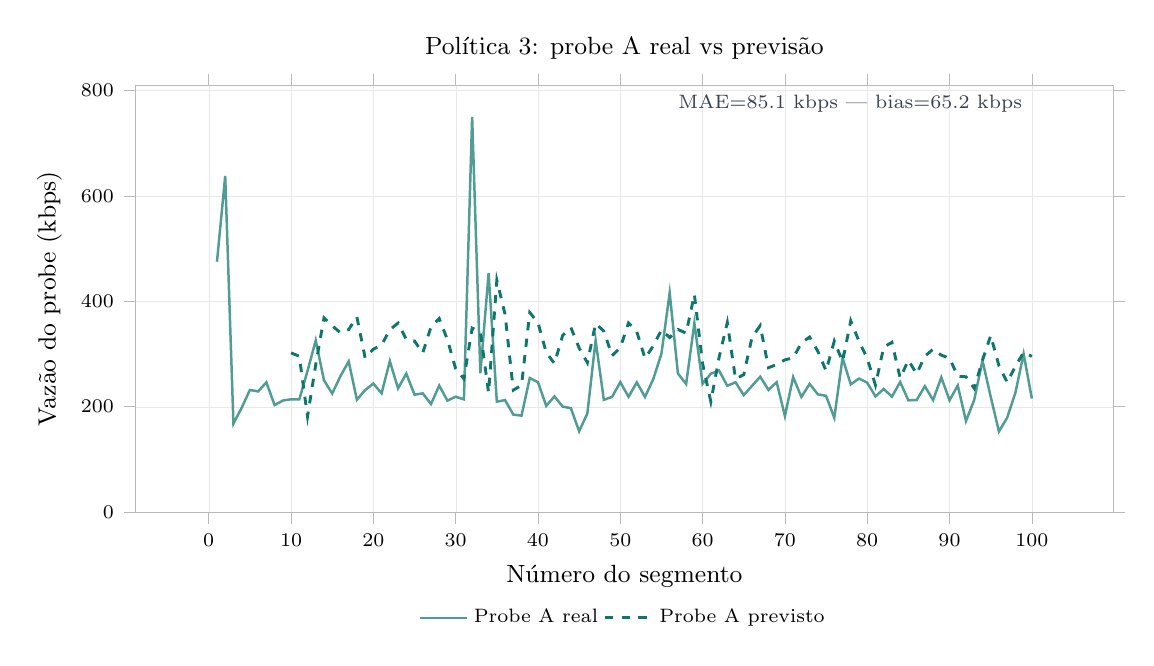
\begin{tikzpicture}
\begin{axis}[
    title={Política 3: probe A real vs previsão},
    xlabel={Número do segmento},
    ylabel={Vazão do probe (kbps)},
    width=14cm,
    height=7cm,
    grid=major,
    grid style={line width=.12pt, draw=gray!18},
    axis line style={draw=gray!55},
    tick style={draw=gray!55},
    tick align=outside,
    title style={font=\small},
    label style={font=\small},
    tick label style={font=\scriptsize},
    legend cell align={left},
    legend style={at={(0.5,-0.20)}, anchor=north, legend columns=2, draw=none, font=\scriptsize},
    ymin=0,
    ymax=809.624
]
\addplot+[plotteal, line width=0.9pt, mark=none, opacity=0.72] coordinates {
(1,475.11)
(2,637.723)
(3,167.816)
(4,197.945)
(5,231.763)
(6,228.953)
(7,246.216)
(8,203.099)
(9,211.609)
(10,214.079)
(11,213.77)
(12,267.688)
(13,325.876)
(14,249.984)
(15,225.034)
(16,257.915)
(17,285.869)
(18,213.122)
(19,231.615)
(20,243.763)
(21,225.464)
(22,286.306)
(23,234.728)
(24,262.771)
(25,222.818)
(26,225.261)
(27,205.021)
(28,240.092)
(29,211.504)
(30,218.959)
(31,213.835)
(32,749.652)
(33,263.251)
(34,453.349)
(35,209.556)
(36,212.506)
(37,185.012)
(38,182.996)
(39,254.404)
(40,246.538)
(41,201.504)
(42,219.538)
(43,200.163)
(44,197.043)
(45,153.192)
(46,187.331)
(47,325.874)
(48,213.016)
(49,218.637)
(50,246.589)
(51,218.848)
(52,246.181)
(53,218.453)
(54,252.097)
(55,300.641)
(56,416.129)
(57,262.982)
(58,243.056)
(59,358.482)
(60,243.484)
(61,262.555)
(62,268.575)
(63,239.624)
(64,246.442)
(65,221.929)
(66,239.474)
(67,256.904)
(68,231.901)
(69,246.472)
(70,182.338)
(71,256.074)
(72,218.51)
(73,243.255)
(74,223.471)
(75,220.567)
(76,178.97)
(77,292.638)
(78,242.357)
(79,253.365)
(80,245.482)
(81,219.398)
(82,233.68)
(83,218.983)
(84,246.812)
(85,212.106)
(86,212.546)
(87,238.827)
(88,212.509)
(89,255.59)
(90,212.23)
(91,240.17)
(92,172.769)
(93,212.93)
(94,287.746)
(95,218.903)
(96,152.996)
(97,179.018)
(98,226.301)
(99,300.3)
(100,215.469)
};
\addlegendentry{Probe A real}
\addplot+[plotteal, dashed, line width=1.05pt, mark=none] coordinates {
(10,301.986)
(11,295.849)
(12,181.36)
(13,280.088)
(14,368.555)
(15,353.53)
(16,340.236)
(17,346.42)
(18,370.208)
(19,292.577)
(20,309.248)
(21,316.988)
(22,346.035)
(23,358.628)
(24,327.754)
(25,324.59)
(26,301.972)
(27,351.466)
(28,367.238)
(29,327.099)
(30,271.932)
(31,253.097)
(32,349.156)
(33,341.899)
(34,226.536)
(35,439.987)
(36,375.43)
(37,231.34)
(38,240.745)
(39,378.604)
(40,359.45)
(41,302.792)
(42,282.048)
(43,335.347)
(44,350.254)
(45,311.263)
(46,283.37)
(47,357.903)
(48,343.282)
(49,296.833)
(50,311.932)
(51,358.959)
(52,342.462)
(53,291.944)
(54,315.198)
(55,345.599)
(56,331.256)
(57,346.551)
(58,339.56)
(59,413.051)
(60,281.682)
(61,209.507)
(62,293.351)
(63,359.614)
(64,252.672)
(65,260.687)
(66,331.439)
(67,353.912)
(68,273.948)
(69,280.032)
(70,288.93)
(71,292.509)
(72,320.858)
(73,332.213)
(74,305.24)
(75,268.04)
(76,324.534)
(77,285.573)
(78,362.974)
(79,324.042)
(80,291.628)
(81,240.875)
(82,312.831)
(83,322.199)
(84,254.338)
(85,288.158)
(86,262.281)
(87,295.597)
(88,309.163)
(89,297.67)
(90,292.147)
(91,257.545)
(92,256.786)
(93,234.791)
(94,287.872)
(95,334.971)
(96,277.834)
(97,246.232)
(98,276.385)
(99,303.124)
(100,295.502)
};
\addlegendentry{Probe A previsto}
\node[anchor=north east, font=\scriptsize, plotgray] at (axis cs:100,809.624) {MAE=85.1 kbps | bias=65.2 kbps};
\end{axis}
\end{tikzpicture}
